%\begin{figure}[!htbp]
%    \centering
%    \caption{}
%    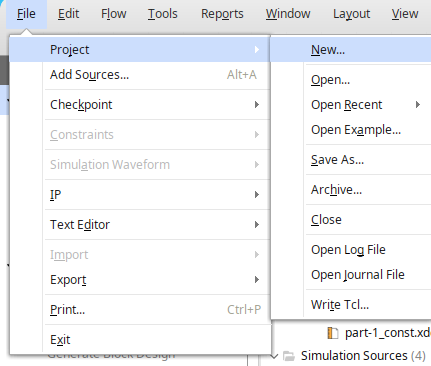
\includegraphics[width=0.5\textwidth]{figure_3_1.png}
%    \label{Figure 3.1}
%\end{figure}\newline

%\begin{center}
%    Truth Table 1: AND Gate Waveform
%    \begin{displaymath}
%    \begin{array}{|c c|c|}
%    In1 & In2 & In1 \land In2\\
%    \hline
%    F & F & F\\
%    F & T & F\\
%    T & F & F\\
%    T & T & T\\
%    \end{array}
%    \end{displaymath}
%\end{center}

\documentclass{article}
\usepackage{graphicx} % Required for inserting images
\usepackage{varwidth}
\usepackage{karnaugh-map}
\usepackage{subfig}
\usepackage{xcolor}
\usepackage{listings}

\captionsetup[lstlisting]{labelformat=empty} % Completely removes "Listing #"
\lstdefinestyle{Verilog}{
  language=Verilog,
  basicstyle=\ttfamily\small,
  keywordstyle=\color{blue}\bfseries,
  commentstyle=\color{gray},
  stringstyle=\color{purple},
  numbers=left,
  numberstyle=\tiny,
  stepnumber=1,
  numbersep=5pt,
  tabsize=2,
  breaklines=true,
  captionpos=b,
  frame=single
}

\title{Experiment 3 Lab Report \\ \large EEE3342C - 00012}
\author{Yousef Awad}
\date{January 2025}
\setcounter{secnumdepth}{0}

\begin{document}

\maketitle
\tableofcontents
\newpage

\section{Equipment}
For this experiment a Windows 11 computer was used alongside the Xilinx Vivado 2024.2 software, alongside an FPGA board, the BASYS 3 development board. The board specifically only used to ensure the simulation by the Vivado software was accurate in the real world, as well as to verify the simulation software wasn't incorrect.\\


\section{Objective}
The objective for this lab was to show how optimizations could be done, as well as to show how circuit area cost is calculated by the Vivado Software. This experiment specifically introduces the concepts of Sums of Products (SOPs) and Products of Sums (POSs), of which are crucial in doing basic simplification of circuits, helping to make a 2 layered circuit diagram possible for boolean equations. Alongside showcasing a way to form those SOPs and POSs via a Karnaugh Map.


\section{Part 1}
\subsection{Simplification of Boolean Expressions}
\subsubsection{AB'C + A'BC' + A'B'C}
The given equation to simplify is the following: $$A*B'*C + A'*B*C' + A'*B'*C$$\\
The simplification process would look like the following:
$$A*B'*C + A'*B*C' + A'*B'*C\rightarrow$$
$$A*B'*C + A'*B'*C + A'*B*C'\rightarrow$$
$$B'*(A*C + A'*C) + A'*B*C'\rightarrow$$
$$B'*C*(A + A') + A'*B*C'\rightarrow$$
$$B'*C*(1) + A'*B*C'\rightarrow$$
$$B'*C + A'*B*C'\rightarrow$$
$$(B'*C + B*C') + (B'*C + A')\rightarrow$$
$$(B \oplus C) + (B'*C + A')\rightarrow$$
$$(B \oplus C) + (B'*C + A')\rightarrow$$
$$(B \oplus C) + B'*C + A'$$
With the following being as far as I can simplify the given equation:
$$(B \oplus C) + B'*C + A'$$
\subsubsection{ABC + AB'C + A'BC' + A'B'C}
The given equation to simplify is the following: $$A*B*C + A*B'*C + A'*B*C' + A'*B'*C$$\\
The simplification process would look like the following:
$$A*B*C + A*B'*C + A'*B*C' + A'*B'*C\rightarrow$$
$$C*(A*B + A*B' + A'*B') + A'*B*C'\rightarrow$$
$$C*(A*B + B'*(A + A')) + A'*B*C'\rightarrow$$
$$C*(A*B + B'*(1)) + A'*B*C'\rightarrow$$
$$C*(A*B + B') + A'*B*C'\rightarrow$$
$$C*((B' + A)*(B' + B)) + A'*B*C'\rightarrow$$
$$C*((B' + A)*(1)) + A'*B*C'\rightarrow$$
$$C*(B' + A) + A'*B*C'\rightarrow$$
$$C*(B' + A) + A'*B*C'\rightarrow$$
$$B'*C + A*C + A'*B*C'$$
With the following being as far as I can simplify the given equation:
$$B'*C + A*C + A'*B*C'$$
\subsection{Find the POS and SOP of the given Truth Table}
Given truth table:
\begin{center}
    \begin{displaymath}
    \begin{array}{|c c c|c|}
      A & B & C & F \\
    \hline
      F & F & F & F \\
      F & F & T & T \\
      F & T & F & F \\
      F & T & T & F \\
      T & F & F & T \\
      T & F & T & T \\
      T & T & F & F \\
      T & T & T & T \\
    \end{array}
    \end{displaymath}
\end{center}
I derived the following sum of products gained from looking at where the result is 1/True, unsimplified:
$$ A'*B'*C + A*B'*C' + A*B'*C + A*B*C $$
I then derived the following product of sums by looking at the output being 0/False and then negating the result, gaining this unsimplified form before and after DeMorgan's Law is applied:
$$ (A'*B'*C' + A'*B*C' + A'*B*C + A*B*C')' \rightarrow$$
$$ (A+B+C)(A+B'+C)(A+B'+C')(A'+B'+C) $$


\section{Part 2}
Given the following truth table:
\begin{center}
    \begin{displaymath}
    \begin{array}{|c c c|c|}
      A & B & C & F \\
    \hline
      F & F & F & F \\
      F & F & T & T \\
      F & T & F & T \\
      F & T & T & F \\
      T & F & F & F \\
      T & F & T & T \\
      T & T & F & T \\
      T & T & T & T \\
    \end{array}
    \end{displaymath}
\end{center}
I derived the following maxterm equation:
$$ A'*B'*C + A'*B*C' + A*B'*C + A*B*C' + A*B*C $$
Of which we can then simplify as shown below:\newline
\begin{centering}
  \begin{displaymath}
  \begin{array}{c | c}
    A'*B'*C + A'*B*C' + A*B'*C + A*B*C' + A*B*C & $Start$ \\
    A'*(B'*C + B*C') + A*(B'*C + B*(C' + C))    & $ Distributive Law $ \\
    A'*(B'*C + B*C') + A*(B'*C + B*(1))         & $ Inverse Law $ \\
    A'*(B'*C + B*C') + A*(B'*C + B)         & $ Identity Law $ \\
    A'*(B \oplus C) + A*(B'*C + B)              & $ XOR Law $ \\
    A'*(B \oplus C) + A*((B + B')(B + C))       & $ Distributive Law $ \\
    A'*(B \oplus C) + A*((1)(B + C))            & $ Inverse Law $ \\
    A'*(B \oplus C) + A*(B + C)                 & $ Identity Law $ \\
    A'*(B \oplus C) + A*B + A*C                 & $ Distributive Law $ \\
  \end{array}
  \end{displaymath}
\end{centering}
With the final simplification being:
$$ A'*(B \oplus C) + A*B + A*C $$
After coding the simplified boolean expression into Verilog, and generating the waveform to double check with the truth table above:
\begin{figure}[!htbp]
    \centering
    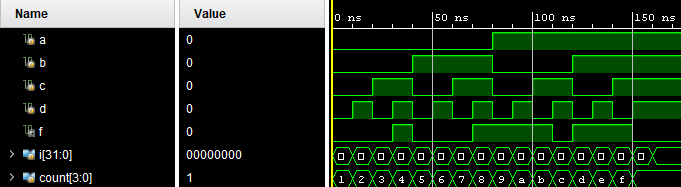
\includegraphics[width=0.5\textwidth]{part-2-waveform.png}
    \label{Part 2 Waveform}
\end{figure}\newline
And, of which, gets the following schematic, with the before schematic being shown to the left of it:
\begin{figure}[!htbp]
    \centering
    \subfloat[\centering Before Schematic]{{ 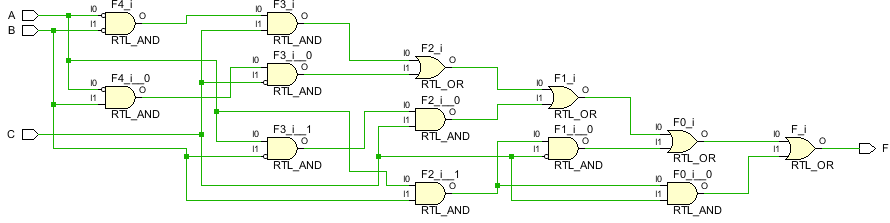
\includegraphics[width=0.4\textwidth]{part-2-schematic-after.png} }}
    \qquad
    \subfloat[\centering After Schematic]{{ 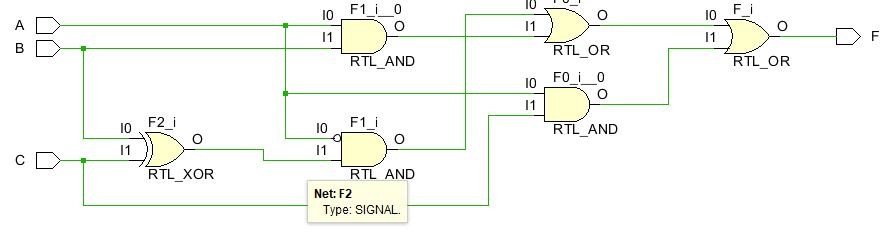
\includegraphics[width=0.4\textwidth]{part-2-schematic-before.png} }}
\end{figure}\newpage
Of which, the verilog code for the before and after schematics is the following:
\begin{lstlisting}[caption={Part 2 Verilog Code}, label={Part 2 Verilog}, style=Verilog]
module before(
        input A, B, C,
        output F
    );
   
    assign F = ~A & ~ B & C | ~A & B & ~C | A & ~B & C | A & B & ~C | A & B & C;
endmodule

module after(
        input A, B, C,
        output F
    );
   
    assign F = ~A & (B ^ C) | A & B | A & C;
endmodule
\end{lstlisting}\newpage
And utilized the following testbench to ensure that it was correct via the waveform above:
\begin{lstlisting}[caption={Part 2 Testbench}, label={Part 2 Testbench}, style=Verilog]
module part_2_sim();
    parameter NUMIN = 4;
    reg[NUMIN - 1:0] count;
    integer i;
    
    reg a, b, c, d;
    wire f;
    
    // replace before with after to check that schematic out
    before UUT(.A(a), .B(b), .C(c), .D(d), .OUT(f));
    
    initial begin
        count = 0;
        for (i = 0; i < 2**NUMIN; i = i + 1) begin
            assign a = count[3];
            assign b = count[2];
            assign c = count[1];
            assign d = count[0];
            
            count = count + 1;
            #10;
        end
    end
    
endmodule
\end{lstlisting}


\section{Part 3}
Given the following truth table:
\begin{figure}[!htbp]
    \centering
    \begin{displaymath}
    \begin{array}{|c c c c|c|}
      A & B & C & D & F \\
    \hline
      F & F & F & F & F \\
      F & F & F & T & F \\
      F & F & T & F & T \\
      F & F & T & T & F \\
      F & T & F & F & F \\
      F & T & F & T & F \\
      F & T & T & F & T \\
      F & T & T & T & T \\
      T & F & F & F & F \\
      T & F & F & T & F \\
      T & F & T & F & T \\
      T & F & T & T & F \\
      T & T & F & F & F \\
      T & T & F & T & F \\
      T & T & T & F & F \\
      T & T & T & T & F \\
    \end{array}
    \end{displaymath}
\end{figure}
We have to find out the funny equation. Therefore doing a simple addition of all of the 1s I get the following result:
$$ A'*B'*C*D' + A'*B*C*D' + A'*B*C*D + A*B'*C*D' $$
And with the following simplification path we can get the Sums of Product form:
\begin{centering}
  \begin{displaymath}
  \begin{array}{c | c}
    A'*B'*C*D' + A'*B*C*D' + A'*B*C*D + A*B'*C*D' & $Start$ \\
    B'*C*D'*(A' + A) + A'*B*C*D' + A'*B*C*D & $Distributive Law$ \\
    B'*C*D'*(1) + A'*B*C*D' + A'*B*C*D & $Complement Law$ \\
    B'*C*D' + A'*B*C*D' + A'*B*C*D & $Identity Law$ \\
    B'*C*D' + A'*B*C*(D' + D) & $Distributive Law$ \\
    B'*C*D' + A'*B*C*(1) & $Complement Law$ \\
    B'*C*D' + A'*B*C & $Identity Law$ \\
    C*(B'*D' + A'*B) & $Distributive Law$ \\
  \end{array}
  \end{displaymath}
\end{centering}
\begin{lstlisting}[caption={Part 3 Verilog Code}, label={Part 3 Verilog}, style=Verilog]
module before(
    assign A, B, C, D,
    output F
  );

  assign F = ~A&~B&C&~D | ~A&B&C&~D | ~A&B&C&D | A&~B&C&~D;

endmodule

module simplified(
    input A, B, C, D,
    output F
  );
 
  assign F = C & (~B & ~D | ~A & B);

endmodule
\end{lstlisting}\newpage
And utilized the following testbench:
\begin{lstlisting}[caption={Part 3 Testbench}, label={Part 3 Testbench}, style=Verilog]
module part_3_sim();
    parameter NUMIN = 4;
    reg[NUMIN - 1:0] count;
    integer i;
    
    reg a, b, c, d;
    wire f;

    // change simplified to before for the before schematic
    simplified UUT(.A(a), .B(b), .C(c), .D(d), .OUT(f)); 
    
    initial begin
        count = 0;
        for (i = 0; i < 2**NUMIN; i = i + 1) begin
            assign a = count[3];
            assign b = count[2];
            assign c = count[1];
            assign d = count[0];
            
            count = count + 1;
            #10;
        end
    end
    
endmodule
\end{lstlisting}
Of which then compiles to the following schematics:
\begin{figure}[!htbp]
    \centering
    \subfloat[\centering Before Schematic]{{ 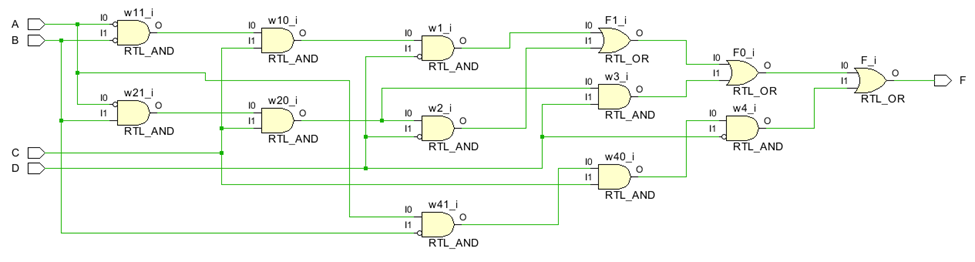
\includegraphics[width=0.5\textwidth]{part-3-schem-before.png} }}
    \qquad
    \subfloat[\centering After Schematic]{{ 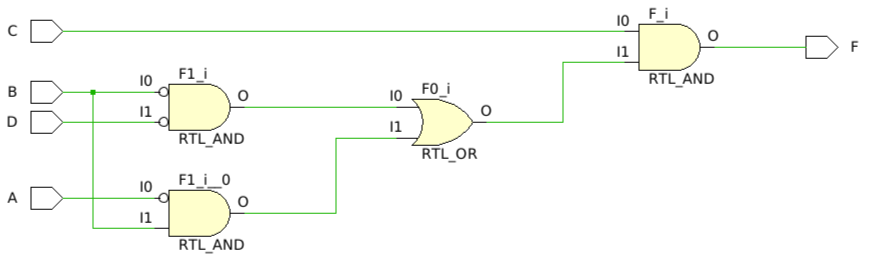
\includegraphics[width=0.5\textwidth]{part-3-schem-after.png} }}
\end{figure}
Of which then provides the following waveform, lining up with the truth table given in the lab manual:
\begin{figure}[!htbp]
    \centering
    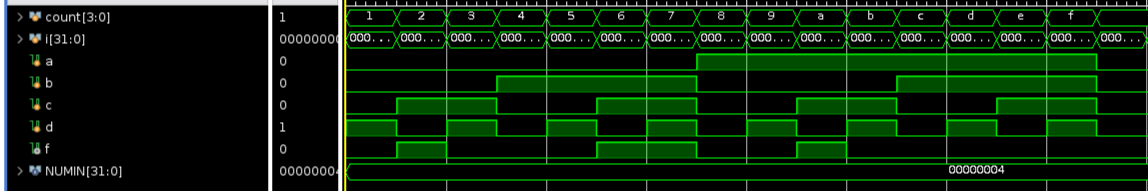
\includegraphics[width=0.75\textwidth]{part-3-waveform.png}
    \label{Part 2 Waveform}
\end{figure}

\newpage
\section{Part 4}
Given the following table for a function we are to create a Karnaugh map and then create it in Verilog.
\begin{figure}[!htbp]
    \centering
    \begin{displaymath}
    \begin{array}{|c c c c|c|}
      A & B & C & D & F \\
    \hline
      F & F & F & F & F \\
      F & F & F & T & F \\
      F & F & T & F & T \\
      F & F & T & T & F \\
      F & T & F & F & F \\
      F & T & F & T & T \\
      F & T & T & F & T \\
      F & T & T & T & T \\
      T & F & F & F & F \\
      T & F & F & T & F \\
      T & F & T & F & T \\
      T & F & T & T & F \\
      T & T & F & F & T \\
      T & T & F & T & T \\
      T & T & T & F & F \\
      T & T & T & T & F \\
    \end{array}
    \end{displaymath}
\end{figure}\\
Therefore, to start with the Karnaugh Map, we need to make it!\\
\begin{karnaugh-map}[4][4][1][$CD$][$AB$]
  \maxterms{0, 1, 3, 4, 8, 9, 11, 14, 15}
  \minterms{2, 5, 6, 7, 10, 12, 13}
  \implicant{2}{6}
  \implicant{5}{7}
  \implicant{12}{13}
  \implicantedge{2}{2}{10}{10}
\end{karnaugh-map}\\
Of which we then have to derive the Minterm (Sums of Products) from the 1 terms of which is the following:
$$ A'*C*D' + A'*B*D + A*B*C' + B'*C*D' $$\\
Of which then we need to get the Maxterm which is the negation of the sum of products form of the 0s:\\
\begin{centering}
  \begin{displaymath}
  \begin{array}{c | c}
    \neg(B'*C'*D' + A'*C'*D' + D*A'*B' + C*A*B + D*A*B') & $MaxTerm Start$ \\
    (B+C+D)(A+C+D)(D'+A+B)(C'+A'+B')(D'+A'+B) & $DeMorgan's Law$ \\
  \end{array}
  \end{displaymath}
\end{centering}\\
Now, when entering into Verilog so as to confirm with the schematic and waveform, you get the following:
\begin{lstlisting}[caption={Part 4 Verilog Code}, label={Part 4 Verilog}, style=Verilog]
module part_4_pos(
        input A, B, C, D,
        output OUT
    );

    assign OUT = (B|C|D)&(A|C|D)&(~D|A|B)&(~C|~A|~B)&(~D|~A|B);

endmodule

module part_4_sop(
        input A, B, C, D,
        output OUT
    );

    assign OUT = (~A&C&~D)|(~A&B&D)|(A&B&~C)|(~B&C&~D);

endmodule
\end{lstlisting}
And got the following schematics for both:
\begin{figure}[!htbp]
    \centering
    \subfloat[\centering Sum of Products Schematic]{{ 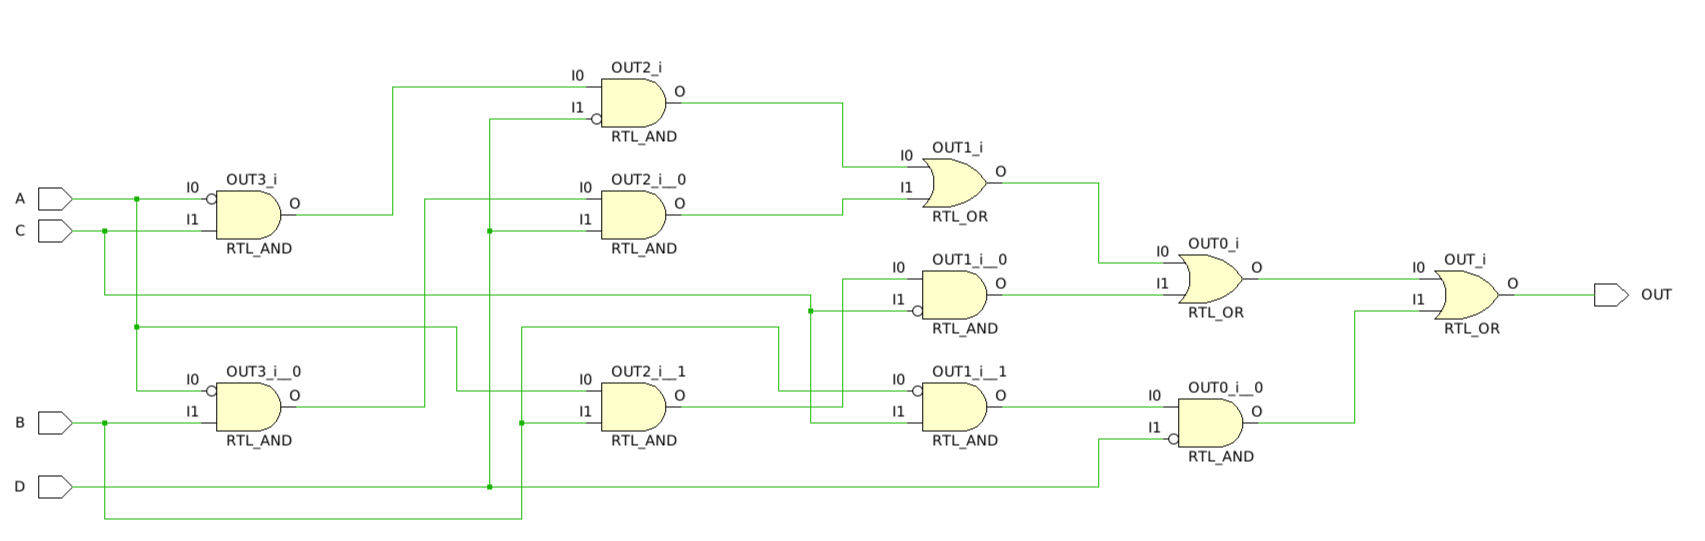
\includegraphics[width=0.5\textwidth]{part-4-schem-sop.png} }}
    \qquad
    \subfloat[\centering Products of Sums Schematic]{{ 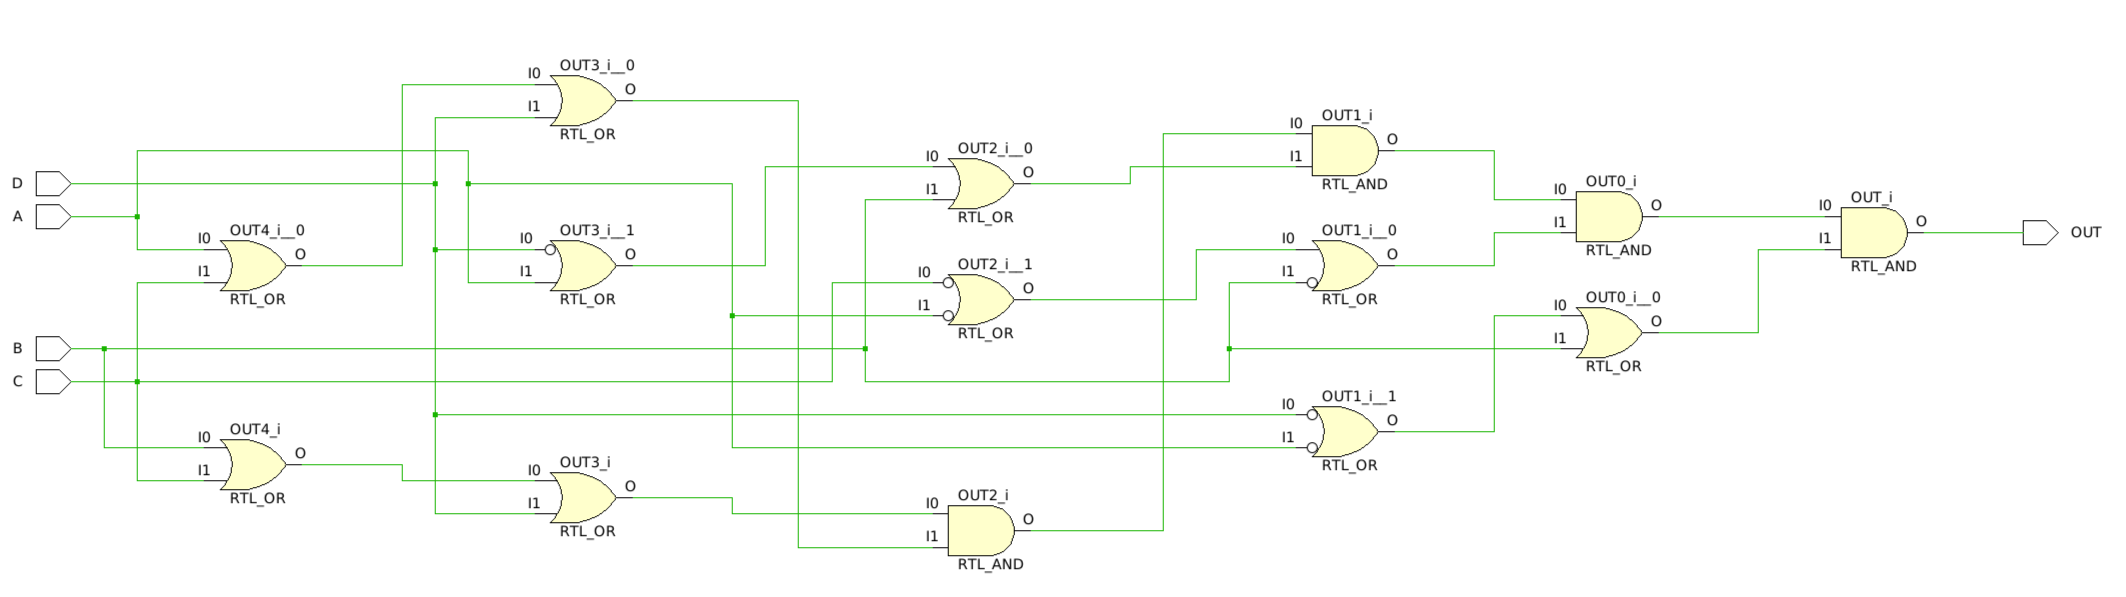
\includegraphics[width=0.5\textwidth]{part-4-schem-pos.png} }}
\end{figure}\\
\begin{figure}[!htbp]
    \centering
    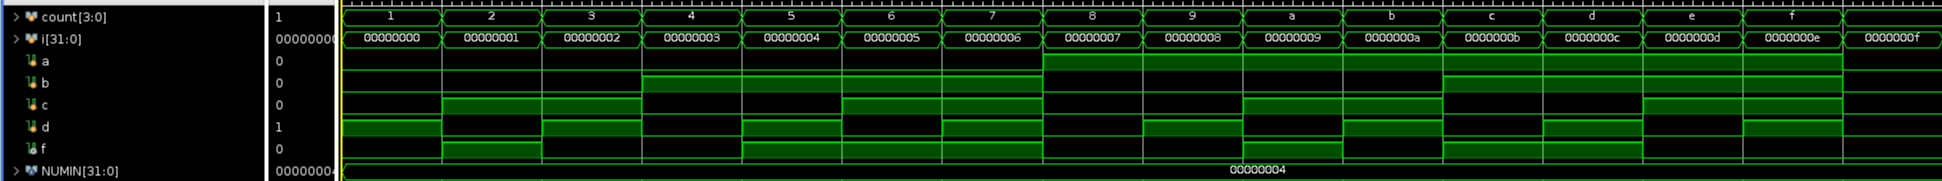
\includegraphics[width=0.75\textwidth]{part-4-waveform.png}
    \label{Part 2 Waveform}
\end{figure}\\
And, with the following testbench below generated the waveform above.
\begin{lstlisting}[caption={Part 4 Testbench}, label={Part 4 Testbench}, style=Verilog]
module part_4_sim();
    parameter NUMIN = 4;
    reg[NUMIN - 1:0] count;
    integer i;
    
    reg a, b, c, d;
    wire f;
    
    part_4_pos UUT(.A(a), .B(b), .C(c), .D(d), .OUT(f));
    
    initial begin
        count = 0;
        for (i = 0; i < 2**NUMIN; i = i + 1) begin
            assign a = count[3];
            assign b = count[2];
            assign c = count[1];
            assign d = count[0];
            
            count = count + 1;
            #10;
        end
    end
    
endmodule
\end{lstlisting}


\newpage
\section{Part 5}
We are given a 4-input system of A, B, C, and D with the following truth table:
\begin{figure}[!htbp]
    \centering
    \begin{displaymath}
    \begin{array}{|c c c c|c|}
      A & B & C & D & OUTPUT \\
    \hline
      F & F & F & F & X \\
      F & F & F & T & F \\
      F & F & T & F & F \\
      F & F & T & T & T \\
      F & T & F & F & X \\
      F & T & F & T & F \\
      F & T & T & F & F \\
      F & T & T & T & T \\
      T & F & F & F & T \\
      T & F & F & T & T \\
      T & F & T & F & T \\
      T & F & T & T & F \\
      T & T & F & F & X \\
      T & T & F & T & T \\
      T & T & T & F & X \\
      T & T & T & T & F \\
    \end{array}
    \end{displaymath}
\end{figure}\newline
Of which then would be converted to the following Karnaugh Map:\newline
\begin{karnaugh-map}[4][4][1][$CD$][$AB$]
  \minterms{3, 7, 8, 9, 10, 13}
  \maxterms{1, 2, 5, 6, 11, 15}
  \indeterminants{0, 4, 12, 14}
  \implicant{12}{9}
  \implicant{3}{7}
  \implicantedge{12}{8}{14}{10}
\end{karnaugh-map}\newpage
After which we will then get the Sum of Product form from the 1-values on the above Karnaugh Map:
$$ A*D' + A'*C*D + A*C' $$
Of which for the Products of Sum form, we get it from the 0-values on the above Karnaugh Map, via ignoring the shaded regions on the map:
$$ \neg(A'*C' + A*C*D + A'*C*D') $$
After which we must then negate it using DeMorgan's Law as well as simplify it to be a Product of Sums:
\begin{centering}
  \begin{displaymath}
  \begin{array}{c | c}
    \neg(A'*C' + A*C*D + A'*C*D') & $Start$ \\
    (A + C) * (A' + C' + D') * (A + C' + D) & $DeMorgan's Law$ \\
  \end{array}
  \end{displaymath}
\end{centering}
Of which then gives us our final result for the Product of Sums form:
$$ (A + C) * (A' + C' + D') * (A + C' + D) $$
Now, to convert them into the Verilog code, so as to verify that they are correct via the waveform, as well as to see the schematic forms. The verilog code would be the following:
\begin{lstlisting}[caption={Part 5 Verilog Code}, label={Part 5 Verilog}, style=Verilog]
module sop(
        input A, B, C, D,
        output F
    );
   
    assign F = A & ~D | ~A & C & D | A & ~ C;

endmodule

module pos(
        input A, B, C, D,
        output F
    );
   
    assign F = (A | C) & (~A | ~C | ~D) & (A | ~C | D);

endmodule
\end{lstlisting}
And of which generated the following waveform, and 2 schematics:
\begin{figure}[!htbp]
    \centering
    \subfloat[\centering Waveform for both Schematics]{{ 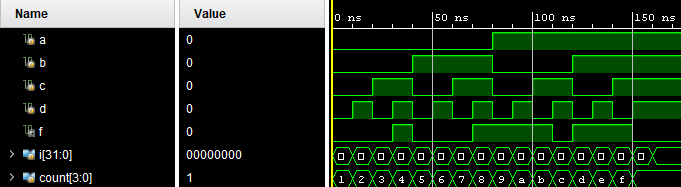
\includegraphics[width=0.5\textwidth]{part-5-waveform.png} }}
\end{figure}\newline
\begin{figure}[!htbp]
    \centering
    \subfloat[\centering Sums of Products Schematic]{{ 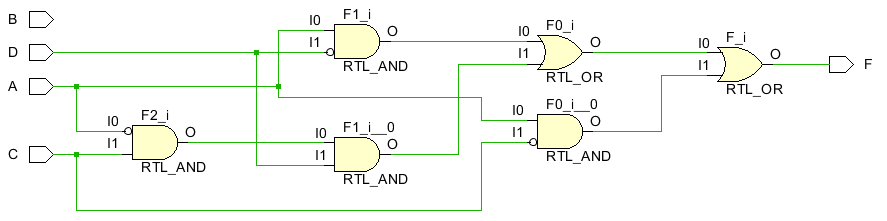
\includegraphics[width=0.4\textwidth]{part-5-schematic-sop.png} }}
    \qquad
    \subfloat[\centering Product of Sums Schematic]{{ 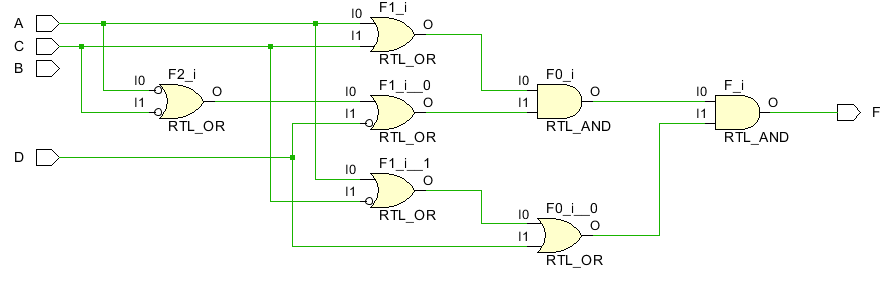
\includegraphics[width=0.4\textwidth]{part-5-schematic-pos.png} }}
\end{figure}\newpage
Of which were generated via the following testbench:
\begin{lstlisting}[caption={Part 5 Testbench}, label={Part 5 Testbench}, style=Verilog]
module part_5_sim();
    parameter NUMIN = 4;
    reg[NUMIN - 1:0] count;
    integer i;
    
    reg a, b, c, d;
    wire f;

    // replace pos with sop for sop form
    part_5_pos UUT(.A(a), .B(b), .C(c), .D(d), .F(f)); 
    
    initial begin
        count = 0;
        for (i = 0; i < 2**NUMIN; i = i + 1) begin
            assign a = count[3];
            assign b = count[2];
            assign c = count[1];
            assign d = count[0];
            
            count = count + 1;
            #10;
        end
    end
    
endmodule
\end{lstlisting}\newpage
\section{Conclusion}
The entire experiment was a glaring success. The results were perfectly as expected, and all tests/checks agreed with one another harmoniously. Alongside this, the testing of the gate logic helped with my understanding of how they function as well as cemented them with the lab reports summarization.
\end{document}
